\documentclass[12pt]{article}\usepackage[]{graphicx}\usepackage[]{xcolor}
% maxwidth is the original width if it is less than linewidth
% otherwise use linewidth (to make sure the graphics do not exceed the margin)
\makeatletter
\def\maxwidth{ %
  \ifdim\Gin@nat@width>\linewidth
    \linewidth
  \else
    \Gin@nat@width
  \fi
}
\makeatother

\definecolor{fgcolor}{rgb}{0.345, 0.345, 0.345}
\newcommand{\hlnum}[1]{\textcolor[rgb]{0.686,0.059,0.569}{#1}}%
\newcommand{\hlstr}[1]{\textcolor[rgb]{0.192,0.494,0.8}{#1}}%
\newcommand{\hlcom}[1]{\textcolor[rgb]{0.678,0.584,0.686}{\textit{#1}}}%
\newcommand{\hlopt}[1]{\textcolor[rgb]{0,0,0}{#1}}%
\newcommand{\hlstd}[1]{\textcolor[rgb]{0.345,0.345,0.345}{#1}}%
\newcommand{\hlkwa}[1]{\textcolor[rgb]{0.161,0.373,0.58}{\textbf{#1}}}%
\newcommand{\hlkwb}[1]{\textcolor[rgb]{0.69,0.353,0.396}{#1}}%
\newcommand{\hlkwc}[1]{\textcolor[rgb]{0.333,0.667,0.333}{#1}}%
\newcommand{\hlkwd}[1]{\textcolor[rgb]{0.737,0.353,0.396}{\textbf{#1}}}%
\let\hlipl\hlkwb

\usepackage{framed}
\makeatletter
\newenvironment{kframe}{%
 \def\at@end@of@kframe{}%
 \ifinner\ifhmode%
  \def\at@end@of@kframe{\end{minipage}}%
  \begin{minipage}{\columnwidth}%
 \fi\fi%
 \def\FrameCommand##1{\hskip\@totalleftmargin \hskip-\fboxsep
 \colorbox{shadecolor}{##1}\hskip-\fboxsep
     % There is no \\@totalrightmargin, so:
     \hskip-\linewidth \hskip-\@totalleftmargin \hskip\columnwidth}%
 \MakeFramed {\advance\hsize-\width
   \@totalleftmargin\z@ \linewidth\hsize
   \@setminipage}}%
 {\par\unskip\endMakeFramed%
 \at@end@of@kframe}
\makeatother

\definecolor{shadecolor}{rgb}{.97, .97, .97}
\definecolor{messagecolor}{rgb}{0, 0, 0}
\definecolor{warningcolor}{rgb}{1, 0, 1}
\definecolor{errorcolor}{rgb}{1, 0, 0}
\newenvironment{knitrout}{}{} % an empty environment to be redefined in TeX

\usepackage{alltt}
\usepackage{array}
\usepackage{amsmath}
\usepackage{mathtools}
\usepackage{gensymb}
\usepackage{graphicx}
\usepackage{float}
\usepackage{caption}

\allowdisplaybreaks
\IfFileExists{upquote.sty}{\usepackage{upquote}}{}
\begin{document}
    \title{Title}
    \author{Ryan Coyne}
    \maketitle
    \section*{Introduction}
        In this lab we measure the cooling of solutions of lauric acid and benzoic acid to determine the freezing point depression constant of lauric acid.
    \section*{Theory Discussion}
        When one substance is dissolved into another, a solution is formed. The vapor pressure, boiling point, and freezing point of the solvent are changed by the addition of the solute. These properties are called colligative properties which means that the change to these properties is dependant on the number of of solute particles in solution, but is not dependant on what the solute is. The change in freezing point can be calculated using the equation\
        \begin{equation*}
            \Delta \text{T} = \text{K}_\text{F}m
        \end{equation*}
        where \(\Delta\)T is the amount that the freezing point is depressed by, \(\text{K}_\text{F}\) is the freezing point depression constant, and \(m\) is the molality of the solution.
    \section*{Procedure}
        \begin{enumerate}
            \item Fill a 600 ml beaker half full with water.
            \item Put the beaker on a hot plate on a low setting.
            \item Fill one test tube without about one inch of lauric acid.
            \item Add between 3.00 and 4.00 grams of lauric acid to a test tube. Record the mass that was added.
            \item Add benzoic acid with 10\% of the mass of the lauric acid. The 10\% is approximate so record the mass that was added.
            \item Repeat step 3.
            \item Add benzoic acid with 20\% of the mass of the lauric acid. Record the mass that was added.
            \item Put a thermometer in each test tube and put the test tubes into the water bath.
            \item Heat until they are all melted.
            \item Turn off the hot plate.
            \item When the temperature begins to decrease record the temperatures in one minute intervals for 4 minutes after the last sample has solidified.
        \end{enumerate}
    \section*{Calculations}
\begin{knitrout}
\definecolor{shadecolor}{rgb}{0.969, 0.969, 0.969}\color{fgcolor}
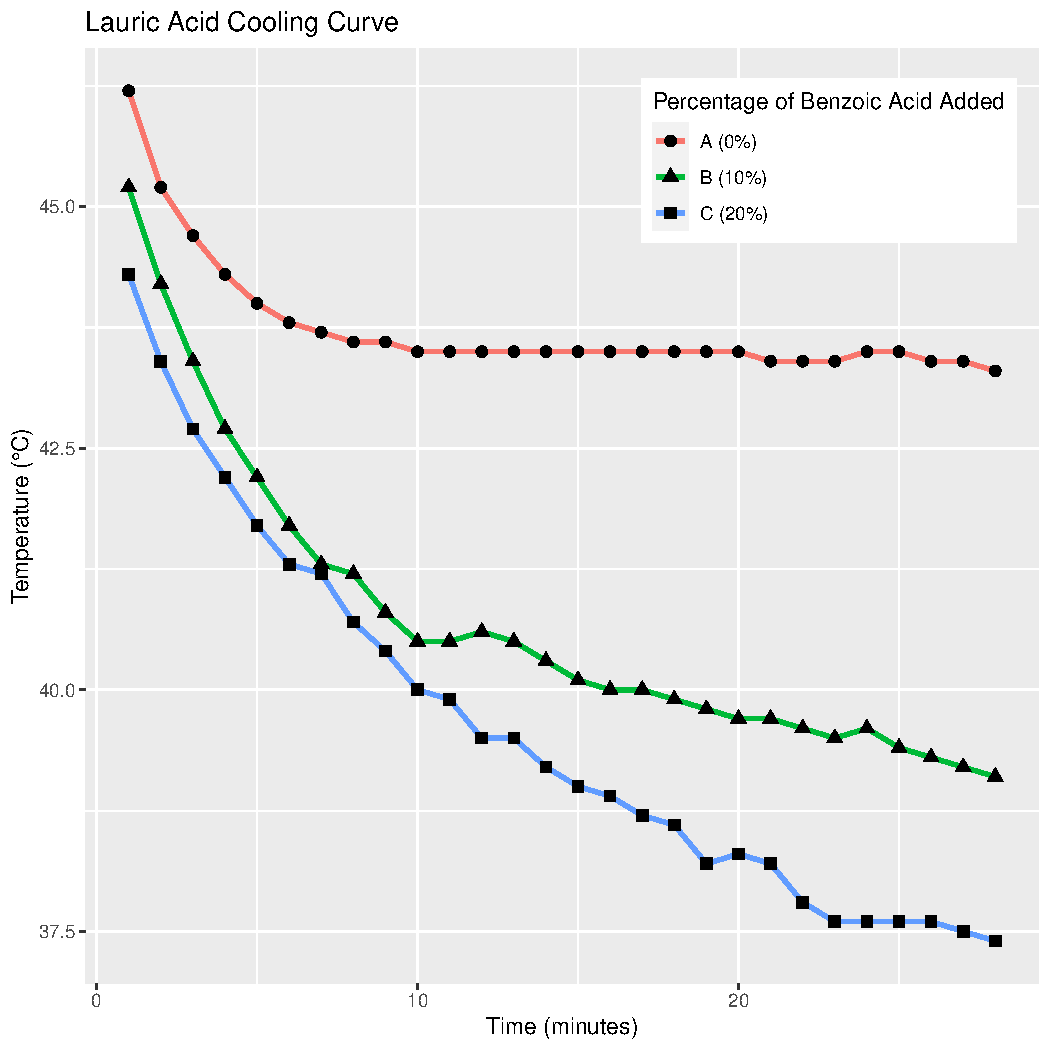
\includegraphics[width=\maxwidth]{figure/coolingPlot-1} 
\end{knitrout}
      \begin{table}[h]
        \centering
        \caption{Mass of Test Tube Samples}
        \begin{tabular}{c|ccc}
            & B (g) & C (g) & D (g)\\
            \hline
            empty & 69.44 & 69.58 & 70.08\\
            w/ lauric acid & 72.52 & 72.61 & 73.12\\
            w/ lauric acid \& benzoic acid & 72.86 & 73.22 & 74.11
        \end{tabular}
    \end{table}
    \begin{align*}
        \text{m}_\text{B} &= 72.52 \text{ g} - 69.44 \text{ g}\\
        &= 3.08 \text{ g}\\
        \text{n}_\text{B} &= (72.86-72.52) \text{ g} \cdot \frac{1 \text{ mole}}{122.13 \text{ g}}\\
        &= 0.00278~\text{moles of benzoic acid}\\
        m_\mathrm{B} &= \frac{0.00278~\text{moles of benzoic acid}}{0.00308\text{ kg}}\\
        &= 0.813 \text{ moles/kg}\\
        \mathrm{K_F} & = \frac{43.5~\mathrm{\degree C} - 40.0~\mathrm{\degree C}}{0.813 \text{ mol/kg}}\\
        &= 3.88~\mathrm{\degree C\cdot kg / mol}\\
        \text{\% error} &= \frac{3.9-3.69}{3.9}\\
        &=1.3\%\\
        \text{m}_\text{C} &= 72.61 \text{ g} - 69.54 \text{ g}\\
        &= 3.07 \text{ g}\\
        \text{n}_\text{C} &= (73.22-72.61) \text{ g} \cdot \frac{1 \text{ mole}}{122.13 \text{ g}}\\
        &= 0.00499~\text{moles of benzoic acid}\\
        m_\mathrm{C} &= \frac{0.00499~\text{moles of benzoic acid}}{0.00307\text{ kg}}\\
        &= 1.63 \text{ moles/kg}\\
        \mathrm{K_F} & = \frac{43.5~\mathrm{\degree C} - 37.6~\mathrm{\degree C}}{1.63 \text{ mol/kg}}\\
        &= 3.62~\mathrm{\degree C\cdot kg / mol}\\
        \text{\%error} &= \frac{3.9-3.62}{3.9}\\
        &= 7.2\%
    \end{align*}
    \section*{Conclusion}
      The goal of this lab was to experimentally determine the freezing point depression constant of lauric acid. To do this we used a sample of lauric acid with beonzoic acid of 10\% of the mass of the lauric acid dissolved in it, and a sample of 20\% beonzoic acid dissolved in it. The freezing point depression constant was measured to be \(3.88~\mathrm{\degree C\cdot kg / mol}\) using the first sample and \(3.62~\mathrm{\degree C\cdot kg / mol}\) using the second sample. The known value is \(3.9~\mathrm{\degree C\cdot kg / mol}\) which means the result from the first sample had an error of 1.3\% and the result from the second had an error of 7.2\%. One source of error could be that the lauric acid was not completely pure and it's mass was therefore not completely accurate.
\end{document}
